\chapter{Análise e discussão dos resultados}

A partir do estudo do processo de produção de biogás através da digestão anaeróbica o grupo discutiu possíveis implementações e custos envolvidos. Foi criado então um cronograma para o detalhamento da proposta e a possível construção de um protótipo para uma análise mais profunda. 

O protótipo a ser construído e estudado será baseado no modelo criado por três estudantes de Engenharia Civil e Engenharia de Produção da Universidade Federal de Alagoas devido ao seu baixo custo e facilidade de construção (NOSSACIENCIA, 2018).
\vspace{0.2cm}

\begin{figure}[htb]
	\begin{center}
	    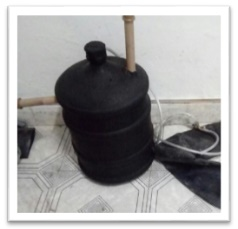
\includegraphics[scale=1.0]{prototipo.jpg}
	\end{center}
	\vspace*{-0.5cm}
	\caption{\label{fig_grafico}Protótipo}
	%\legend{Fonte: \citeonline[p. 24]{araujo2012}}
\end{figure}